\PassOptionsToPackage{quiet}{xeCJK}
\documentclass[answer,fontset=fandol]{THUExam}
\usepackage{HTNotes-math}
\usepackage{pifont}
\usepackage{ulem}

\usepackage{tikz}
\usetikzlibrary{positioning, calc, shapes.geometric, shapes, shapes.multipart, arrows.meta, arrows, decorations.markings, external, trees}

% =================================================
%       PDF信息
% =================================================
\title{高等数学A (二)}
\author{}
\Subject{复习题}
\Keywords{高等数学, 重积分, 二重积分, 三重积分, 极坐标, 变量替换}

% =================================================
%       试卷头信息
% =================================================
\Year{2025--2026}
\Semester{春季}
\Course{高等数学A}
\Time{}
\Type{A}

\begin{document}
\vspace{1cm}
\makehead

\begin{note}
\textbf{常用积分表：}
\[
\begin{array}{ll}
\displaystyle\int k\,\mathrm{d}x=kx+C\ (k\text{ 是常数})&
\displaystyle\int x^\mu\,\mathrm{d}x=\frac{x^{\mu+1}}{\mu+1}+C\ (\mu\neq-1)\\[8pt]
\displaystyle\int\frac{\mathrm{d}x}{x}=\ln|x|+C&
\displaystyle\int\frac{\mathrm{d}x}{1+x^2}=\arctan x+C\\[8pt]
\displaystyle\int\frac{\mathrm{d}x}{\sqrt{1-x^2}}=\arcsin x+C&
\displaystyle\int\cos x\,\mathrm{d}x=\sin x+C\\[8pt]
\displaystyle\int\sin x\,\mathrm{d}x=-\cos x+C&
\displaystyle\int\sec^2x\,\mathrm{d}x=\tan x+C\\[8pt]
\displaystyle\int\csc^2x\,\mathrm{d}x=-\cot x+C&
\displaystyle\int\sec x\tan x\,\mathrm{d}x=\sec x+C\\[8pt]
\displaystyle\int\csc x\cot x\,\mathrm{d}x=-\csc x+C&
\displaystyle\int e^x\,\mathrm{d}x=e^x+C\\[8pt]
\displaystyle\int a^x\,\mathrm{d}x=\frac{a^x}{\ln a}+C\ (a>0,\ a\neq1)&
\displaystyle\int\tan x\,\mathrm{d}x=-\ln|\cos x|+C\\[8pt]
\displaystyle\int\cot x\,\mathrm{d}x=\ln|\sin x|+C&
\displaystyle\int\sec x\,\mathrm{d}x=\ln|\sec x+\tan x|+C\\[8pt]
\displaystyle\int\csc x\,\mathrm{d}x=\ln|\csc x-\cot x|+C&
\displaystyle\int\frac{\mathrm{d}x}{a^2+x^2}=\frac1a\arctan\frac{x}{a}+C\\[8pt]
\displaystyle\int\frac{\mathrm{d}x}{x^2-a^2}=\frac{1}{2a}\ln\left|\frac{x-a}{x+a}\right|+C&
\displaystyle\int\frac{\mathrm{d}x}{\sqrt{a^2-x^2}}=\arcsin\frac{x}{a}+C\\[8pt]
\displaystyle\int\frac{\mathrm{d}x}{\sqrt{x^2+a^2}}=\ln\left(x+\sqrt{x^2+a^2}\right)+C&
\displaystyle\int\frac{\mathrm{d}x}{\sqrt{x^2-a^2}}=\ln\left|x+\sqrt{x^2-a^2}\right|+C
\end{array}
\]
\end{note}
\bigskip

% =================================================
%       概念与基本工具
% =================================================
\makepart{概念与基本工具}{重积分的定义、几何意义与常用积分}

\begin{note}
\textbf{二重积分的定义：} 将有界闭区域 $D$ 分成 $n$ 个小区域 $\Delta\sigma_i$，在每个小区域中任取点 $(\xi_i,\eta_i)$。若当最大直径 $\lambda\to0$ 时，极限
\[
\lim_{\lambda\to0}\sum_{i=1}^n f(\xi_i,\eta_i)\Delta\sigma_i
\]
存在，且与分割方法、取点方法无关，则称 $f$ 在 $D$ 上可积，并把该极限记为
\[
\iint_D f(x,y)\,\mathrm{d}\sigma.
\]
当 $f(x,y)\geqslant0$ 时，它表示以 $D$ 为底、以 $z=f(x,y)$ 为顶面的曲顶柱体体积。
\end{note}
\bigskip

\begin{problem}
设 $D$ 是顶点为 $(0,0),(4,0),(3,2),(1,2)$ 的梯形区域，则定高柱体
\[
0\leqslant z\leqslant 5,\qquad (x,y)\in D
\]
的体积为 \fillin{$30$}。
\end{problem}
\begin{note}
遇到常数函数的二重积分，不要急着列累次积分。先看它是不是``定高''：常数高度 $\times$ 平面区域面积，通常更快。
\end{note}
\begin{solution}
梯形的两条平行边长度分别为 $4$ 和 $2$，高为 $2$，故
\[
S_D=\frac{4+2}{2}\cdot2=6.
\]
于是
\[
V=\iint_D5\,\mathrm{d}\sigma=5S_D=\boxed{30}.
\]
\end{solution}
\bigskip

\begin{problem}
平面
\[
\frac{x}{a}+\frac{y}{b}+\frac{z}{c}=1\qquad(a,b,c>0)
\]
和三坐标面所割出的第一卦限内立体的体积为 \fillin{$\dfrac{abc}{6}$}。
\end{problem}
\begin{note}
第一卦限截距式平面与坐标面围成的四面体体积为 $\dfrac{abc}{6}$。课堂上要会积分推导，考试中也可用这个结论快速核对。
\end{note}
\begin{solution}
投影区域为
\[
D=\left\{(x,y)\mid x\geqslant0,\ y\geqslant0,\ \frac{x}{a}+\frac{y}{b}\leqslant1\right\},
\]
顶面为
\[
z=c\left(1-\frac{x}{a}-\frac{y}{b}\right).
\]
于是
\begin{align*}
V
&=\iint_D c\left(1-\frac{x}{a}-\frac{y}{b}\right)\mathrm{d}\sigma\\
&=c\int_0^a\mathrm{d}x\int_0^{b(1-x/a)}
\left(1-\frac{x}{a}-\frac{y}{b}\right)\mathrm{d}y
=\boxed{\frac{abc}{6}}.
\end{align*}
\end{solution}
\bigskip

\begin{note}
\textbf{本讲常用的一维积分表：}
\[
\begin{array}{c|c}
\text{积分} & \text{结果} \\ \hline
\displaystyle\int x^n\,\mathrm{d}x\ (n\neq-1) & \displaystyle\frac{x^{n+1}}{n+1}+C\\[6pt]
\displaystyle\int \sin x\,\mathrm{d}x & -\cos x+C\\[4pt]
\displaystyle\int x^2\sin x\,\mathrm{d}x & -x^2\cos x+2x\sin x+2\cos x+C\\[4pt]
\displaystyle\int\sin^3x\,\mathrm{d}x & -\cos x+\frac{1}{3}\cos^3x+C\\[4pt]
\displaystyle\int r\sqrt{R^2-r^2}\,\mathrm{d}r & -\frac{1}{3}(R^2-r^2)^{3/2}+C\\[6pt]
\displaystyle\int_0^{\pi/2}\sin^3\theta\,\mathrm{d}\theta
=\int_0^{\pi/2}\cos^3\theta\,\mathrm{d}\theta & \displaystyle\frac{2}{3}
\end{array}
\]
\end{note}
\bigskip

\begin{problem}
设
\[
D=\{(x,y)\mid x^2+y^2\leqslant R^2,\ y\geqslant0\}.
\]
则
\[
\iint_D\sqrt{R^2-x^2-y^2}\,\mathrm{d}\sigma
\]
的值为 \fillin{$\dfrac{\pi R^3}{3}$}。
\end{problem}
\begin{solution}
被积函数是上半球面
\[
z=\sqrt{R^2-x^2-y^2}
\]
的高度。若底面取整个圆盘 $x^2+y^2\leqslant R^2$，体积为半球体积
\[
\frac12\cdot\frac{4}{3}\pi R^3=\frac{2}{3}\pi R^3.
\]
现在 $D$ 只是上半圆盘，对称性给出
\[
\iint_D\sqrt{R^2-x^2-y^2}\,\mathrm{d}\sigma
=\frac12\cdot\frac{2}{3}\pi R^3
=\boxed{\frac{\pi R^3}{3}}.
\]
\end{solution}
\bigskip

% =================================================
%       基础计算
% =================================================
\newpage
\makepart{基础计算}{区域识别、对称性与简单累次积分}

\begin{problem}
计算
\[
\iint_D\left(x^2-y^2\right)\mathrm{d}\sigma,\qquad
D=\{(x,y)\mid 0\leqslant y\leqslant \sin x,\ 0\leqslant x\leqslant \pi\}.
\]
\end{problem}
\begin{solution}
直接按区域给出的顺序积分。先对 $y$ 积分：
\begin{align*}
\iint_D(x^2-y^2)\,\mathrm{d}\sigma
&=\int_0^\pi\mathrm{d}x\int_0^{\sin x}(x^2-y^2)\,\mathrm{d}y\\
&=\int_0^\pi\left[x^2y-\frac{y^3}{3}\right]_{0}^{\sin x}\mathrm{d}x\\
&=\int_0^\pi\left(x^2\sin x-\frac{\sin^3x}{3}\right)\mathrm{d}x.
\end{align*}
记
\[
I_1=\int_0^\pi x^2\sin x\,\mathrm{d}x,\qquad
I_2=\int_0^\pi\sin^3x\,\mathrm{d}x.
\]

先计算 $I_1$。这里需要分部积分，取
\[
u=x^2,\qquad \mathrm{d}v=\sin x\,\mathrm{d}x,
\]
则
\[
\mathrm{d}u=2x\,\mathrm{d}x,\qquad v=-\cos x.
\]
因此
\begin{align*}
I_1
&=\left[-x^2\cos x\right]_0^\pi+\int_0^\pi 2x\cos x\,\mathrm{d}x\\
&=\pi^2+2\int_0^\pi x\cos x\,\mathrm{d}x.
\end{align*}
对剩下的积分再次分部积分，取
\[
u=x,\qquad \mathrm{d}v=\cos x\,\mathrm{d}x,
\]
则
\[
\mathrm{d}u=\mathrm{d}x,\qquad v=\sin x.
\]
于是
\[
\int_0^\pi x\cos x\,\mathrm{d}x
=\left[x\sin x\right]_0^\pi-\int_0^\pi\sin x\,\mathrm{d}x
=0-\left[-\cos x\right]_0^\pi=-2.
\]
所以
\[
I_1=\pi^2+2(-2)=\pi^2-4.
\]

再计算 $I_2$：
\[
I_2=\int_0^\pi\sin x(1-\cos^2x)\,\mathrm{d}x.
\]
令 $t=\cos x$，$\mathrm{d}t=-\sin x\,\mathrm{d}x$，当 $x=0$ 时 $t=1$，当 $x=\pi$ 时 $t=-1$，故
\[
I_2=-\int_1^{-1}(1-t^2)\,\mathrm{d}t
=\int_{-1}^{1}(1-t^2)\,\mathrm{d}t
=\left[t-\frac{t^3}{3}\right]_{-1}^{1}
=\frac{4}{3}.
\]

因此
\[
\text{原式}=I_1-\frac{1}{3}I_2
=\pi^2-4-\frac{1}{3}\cdot\frac{4}{3}
=\boxed{\pi^2-\frac{40}{9}}.
\]
\end{solution}
\bigskip

\begin{problem}
计算
\[
\iint_D\left(y^2+3x-6y+5xy+x^3y^2-7xy^4+9\right)\mathrm{d}\sigma,
\]
其中
\[
D=\{(x,y)\mid x^2+y^2\leqslant R^2\}.
\]
\end{problem}
\begin{note}
圆盘、椭圆盘、关于坐标轴对称的区域上，先看奇函数项能不能直接消掉。很多看上去很长的被积函数，真正要算的只剩偶函数项。
\end{note}
\begin{solution}
圆盘 $D$ 关于 $x$ 轴、$y$ 轴均对称，所以
\[
\iint_D3x\,\mathrm{d}\sigma=0,\quad
\iint_D(-6y)\,\mathrm{d}\sigma=0,\quad
\iint_D5xy\,\mathrm{d}\sigma=0,
\]
\[
\iint_Dx^3y^2\,\mathrm{d}\sigma=0,\qquad
\iint_D(-7xy^4)\,\mathrm{d}\sigma=0.
\]
这些项至少关于 $x$ 或 $y$ 中的一个变量为奇函数。又由轮换对称性，
\[
\iint_Dy^2\,\mathrm{d}\sigma
=\frac{1}{2}\iint_D(x^2+y^2)\,\mathrm{d}\sigma.
\]
用极坐标计算
\[
\iint_D(x^2+y^2)\,\mathrm{d}\sigma
=\int_0^{2\pi}\mathrm{d}\theta\int_0^Rr^3\,\mathrm{d}r
=\frac{\pi R^4}{2}.
\]
于是
\[
\text{原式}=\frac{\pi R^4}{4}+9\pi R^2
=\boxed{\pi R^2\left(\frac{R^2}{4}+9\right)}.
\]
\end{solution}
\bigskip

\begin{problem}
计算
\[
\iint_D (x+2y)\,\mathrm{d}\sigma,
\]
其中 $D$ 由抛物线 $y=x^2$、直线 $y=2x$ 和直线 $x=1$ 围成。
\end{problem}
\begin{solution}
区域可写为
\[
0\leqslant x\leqslant1,\qquad x^2\leqslant y\leqslant2x.
\]
于是
\begin{align*}
\iint_D(x+2y)\,\mathrm{d}\sigma
&=\int_0^1\mathrm{d}x\int_{x^2}^{2x}(x+2y)\,\mathrm{d}y\\
&=\int_0^1\left[x y+y^2\right]_{y=x^2}^{2x}\mathrm{d}x\\
&=\int_0^1(6x^2-x^3-x^4)\,\mathrm{d}x\\
&=2-\frac14-\frac15
=\boxed{\frac{31}{20}}.
\end{align*}
\end{solution}
\bigskip

% =================================================
%       交换积分次序
% =================================================
\newpage
\makepart{交换积分次序}{画区域、找边界、必要时拆分}

\begin{note}
\textbf{交换积分次序的固定步骤：}
\begin{enumerate}
	\item 把原积分写成区域不等式；
	\item 把所有边界曲线改写成同一种方向的函数；
	\item 找交点；
	\item 判断固定新外层变量时，内层变量是否需要分段。
\end{enumerate}
不要只凭上下限猜图形，尤其是根号、圆弧和分段区域。
\end{note}
\bigskip

\begin{problem}
交换下列积分的次序：
\[
\int_0^4 \mathrm{d}y \int_{-\sqrt{4-y}}^{\frac{1}{2}(y-4)} f(x,y)\,\mathrm{d}x.
\]
\end{problem}
\begin{solution}
区域为
\[
0\leqslant y\leqslant4,\qquad
-\sqrt{4-y}\leqslant x\leqslant\frac{y-4}{2}.
\]
两条边界分别为
\[
x=-\sqrt{4-y}\Longleftrightarrow y=4-x^2,\qquad
x=\frac{y-4}{2}\Longleftrightarrow y=2x+4.
\]
二者交于 $x=-2,0$，对应点为 $(-2,0)$ 和 $(0,4)$。因此
\[
\boxed{
\int_{-2}^0\mathrm{d}x\int_{2x+4}^{4-x^2}f(x,y)\,\mathrm{d}y
}.
\]
\end{solution}
\bigskip

\begin{problem}
交换下列积分的次序：
\[
\int_0^1 \mathrm{d}x \int_{\sqrt{x}}^{1+\sqrt{1-x^2}} f(x,y)\,\mathrm{d}y.
\]
\end{problem}
\begin{solution}
区域为
\[
0\leqslant x\leqslant1,\qquad
\sqrt{x}\leqslant y\leqslant1+\sqrt{1-x^2}.
\]
下边界是 $y=\sqrt{x}$，即 $x=y^2$；上边界是上半圆
\[
x^2+(y-1)^2=1,\qquad y\geqslant1.
\]
换成 $y$ 为外层时需要分段：
\[
0\leqslant y\leqslant1:\quad 0\leqslant x\leqslant y^2;
\]
\[
1\leqslant y\leqslant2:\quad 0\leqslant x\leqslant\sqrt{1-(y-1)^2}.
\]
因此
\[
\boxed{
\int_0^1\mathrm{d}y\int_0^{y^2}f(x,y)\,\mathrm{d}x
+\int_1^2\mathrm{d}y\int_0^{\sqrt{1-(y-1)^2}}f(x,y)\,\mathrm{d}x
}.
\]
\end{solution}
\bigskip

\begin{problem}
计算
\[
I=\int_0^1\mathrm{d}x\int_x^1 \cos(y^2)\,\mathrm{d}y.
\]
\end{problem}
\begin{note}
这类题是真正需要交换积分次序的典型：原内层是 $\cos(y^2)$ 对 $y$ 积分，不好算；交换后先对 $x$ 积分，只留下一个因子 $y$，正好配合 $\cos(y^2)$。
\end{note}
\begin{solution}
区域为
\[
0\leqslant x\leqslant1,\qquad x\leqslant y\leqslant1.
\]
交换次序：
\[
0\leqslant y\leqslant1,\qquad 0\leqslant x\leqslant y.
\]
于是
\[
I=\int_0^1\mathrm{d}y\int_0^y \cos(y^2)\,\mathrm{d}x
=\int_0^1 y\cos(y^2)\,\mathrm{d}y
=\boxed{\frac{\sin1}{2}}.
\]
\end{solution}
\bigskip

\begin{problem}
计算
\[
I=\int_0^1\mathrm{d}y\int_y^1 e^{-x^2}\,\mathrm{d}x.
\]
\end{problem}
\begin{solution}
原积分中 $e^{-x^2}$ 对 $x$ 的原函数不属于初等函数。区域为
\[
0\leqslant y\leqslant1,\qquad y\leqslant x\leqslant1.
\]
交换次序得
\[
0\leqslant x\leqslant1,\qquad 0\leqslant y\leqslant x.
\]
于是
\[
I=\int_0^1\mathrm{d}x\int_0^x e^{-x^2}\,\mathrm{d}y
=\int_0^1 xe^{-x^2}\,\mathrm{d}x
=\boxed{\frac{1-e^{-1}}{2}}.
\]
\end{solution}
\bigskip

% =================================================
%       极坐标
% =================================================
\newpage
\makepart{极坐标}{圆、扇形、心形线与角度函数}

\begin{note}
\textbf{极坐标换元：}
\[
x=r\cos\theta,\qquad y=r\sin\theta,\qquad
\mathrm{d}\sigma=r\,\mathrm{d}r\,\mathrm{d}\theta.
\]
当区域边界含有 $x^2+y^2$、圆、扇形、射线，或被积函数含有 $\sqrt{x^2+y^2}$、$\arctan(y/x)$ 时，应优先考虑极坐标。
\end{note}
\bigskip

\begin{problem}
计算
\[
\iint_D \arctan\frac{y}{x}\,\mathrm{d}\sigma,
\]
其中
\[
D=\{(x,y)\mid 1\leqslant x^2+y^2\leqslant4,\ x>0,\ y>0\}.
\]
\end{problem}
\begin{solution}
在第一象限，$\arctan\dfrac{y}{x}=\theta$。区域为
\[
1\leqslant r\leqslant2,\qquad 0\leqslant\theta\leqslant\frac{\pi}{2}.
\]
故
\[
\iint_D \arctan\frac{y}{x}\,\mathrm{d}\sigma
=\int_0^{\pi/2}\mathrm{d}\theta\int_1^2 \theta r\,\mathrm{d}r
=\left[\frac{\theta^2}{2}\right]_0^{\pi/2}\left[\frac{r^2}{2}\right]_1^2
=\boxed{\frac{3\pi^2}{16}}.
\]
\end{solution}
\bigskip

\begin{problem}
计算
\[
\iint_D (x^2+y^2)\,\mathrm{d}\sigma,
\]
其中 $D$ 是由 $r=1+\cos\theta$ 围成的心形线区域。

\begin{center}
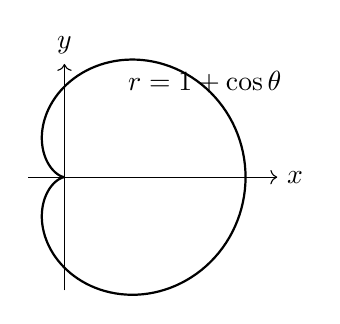
\begin{tikzpicture}[scale=1.15]
  \draw[->] (-0.4,0) -- (2.35,0) node[right] {$x$};
  \draw[->] (0,-1.25) -- (0,1.25) node[above] {$y$};
  \draw[thick,domain=0:360,samples=180,variable=\t]
    plot ({(1+cos(\t))*cos(\t)},{(1+cos(\t))*sin(\t)});
  \node at (1.55,1.05) {$r=1+\cos\theta$};
\end{tikzpicture}
\end{center}
\end{problem}
\begin{solution}
区域为
\[
0\leqslant\theta\leqslant2\pi,\qquad 0\leqslant r\leqslant1+\cos\theta.
\]
被积函数 $x^2+y^2=r^2$，面积元素为 $r\,\mathrm{d}r\,\mathrm{d}\theta$，故
\[
\iint_D(x^2+y^2)\,\mathrm{d}\sigma
=\int_0^{2\pi}\mathrm{d}\theta\int_0^{1+\cos\theta}r^3\,\mathrm{d}r
=\frac14\int_0^{2\pi}(1+\cos\theta)^4\,\mathrm{d}\theta.
\]
利用
\[
\int_0^{2\pi}\cos\theta\,\mathrm{d}\theta=0,\quad
\int_0^{2\pi}\cos^2\theta\,\mathrm{d}\theta=\pi,\quad
\int_0^{2\pi}\cos^4\theta\,\mathrm{d}\theta=\frac{3\pi}{4},
\]
得到
\[
\frac14\int_0^{2\pi}(1+4\cos\theta+6\cos^2\theta+4\cos^3\theta+\cos^4\theta)\mathrm{d}\theta
=\frac14\left(2\pi+6\pi+\frac{3\pi}{4}\right)
=\boxed{\frac{35\pi}{16}}.
\]
\end{solution}
\bigskip

% =================================================
%       变量替换
% =================================================
\newpage
\makepart{变量替换与 Jacobi 行列式}{把弯曲区域变成矩形区域}

\begin{note}
\textbf{二重积分变量替换公式：} 若
\[
x=x(u,v),\qquad y=y(u,v),
\]
且变换一一对应、Jacobi 行列式不为零，则
\[
\iint_D f(x,y)\,\mathrm{d}\sigma
=\iint_{\widetilde D} f(x(u,v),y(u,v))
\left|\frac{\partial(x,y)}{\partial(u,v)}\right|
\mathrm{d}u\,\mathrm{d}v.
\]
关键不是背公式，而是同时变换三件事：被积函数、区域边界、面积元素。
\end{note}
\bigskip

\begin{problem}
计算
\[
\iint_D (x^2-y^2)\,\mathrm{d}\sigma,
\]
其中 $D$ 是由曲线
\[
xy=1,\qquad xy=2,\qquad y=x,\qquad y=4x
\]
在第一象限围成的区域。

\begin{center}
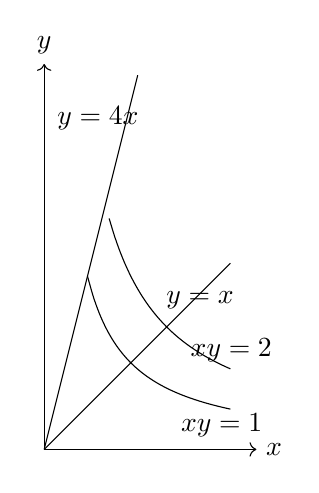
\begin{tikzpicture}[scale=1.1]
  \draw[->] (0,0) -- (2.45,0) node[right] {$x$};
  \draw[->] (0,0) -- (0,4.45) node[above] {$y$};
  \draw[domain=0.5:2.15,smooth,variable=\x] plot ({\x},{1/\x});
  \draw[domain=0.75:2.15,smooth,variable=\x] plot ({\x},{2/\x});
  \draw[domain=0:2.15] plot ({\x},{\x});
  \draw[domain=0:1.08] plot ({\x},{4*\x});
  \node at (2.05,0.28) {$xy=1$};
  \node at (2.16,1.15) {$xy=2$};
  \node at (1.8,1.72) {$y=x$};
  \node at (0.62,3.82) {$y=4x$};
\end{tikzpicture}
\end{center}
\end{problem}
\begin{solution}
令
\[
u=xy,\qquad v=\frac{y}{x}\qquad(x>0,\ y>0).
\]
边界直接变为矩形：
\[
1\leqslant u\leqslant2,\qquad 1\leqslant v\leqslant4.
\]
又
\[
x^2=\frac{u}{v},\qquad y^2=uv,\qquad
x^2-y^2=u\left(\frac1v-v\right).
\]
Jacobi 行列式满足
\[
\frac{\partial(u,v)}{\partial(x,y)}
=
\begin{vmatrix}
y & x\\[2pt]
-\dfrac{y}{x^2} & \dfrac1x
\end{vmatrix}
=2\frac{y}{x}=2v,
\]
所以
\[
\left|\frac{\partial(x,y)}{\partial(u,v)}\right|=\frac{1}{2v}.
\]
因此
\begin{align*}
\iint_D(x^2-y^2)\,\mathrm{d}\sigma
&=\int_1^2\mathrm{d}u\int_1^4
u\left(\frac1v-v\right)\frac{1}{2v}\,\mathrm{d}v\\
&=\frac12\int_1^2u\,\mathrm{d}u
\int_1^4\left(\frac1{v^2}-1\right)\mathrm{d}v\\
&=\frac12\cdot\frac32\cdot
\left[-\frac1v-v\right]_1^4
=\boxed{-\frac{27}{16}}.
\end{align*}
\end{solution}
\bigskip

\begin{problem}
设 $D$ 是由直线
\[
x+y=1,\qquad x+y=3,\qquad y-x=0,\qquad y-x=2
\]
围成的平行四边形。计算
\[
\iint_D (x+y)(y-x)\,\mathrm{d}\sigma.
\]

\begin{center}
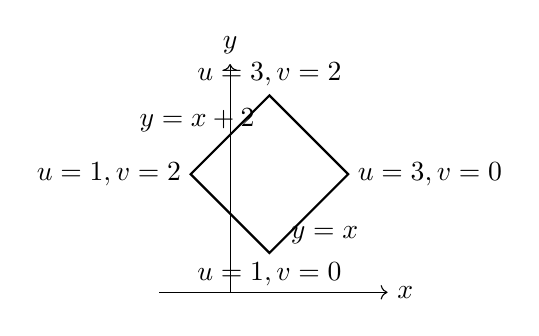
\begin{tikzpicture}[scale=1.0]
  \draw[->] (-0.9,0) -- (2.0,0) node[right] {$x$};
  \draw[->] (0,0) -- (0,2.9) node[above] {$y$};
  \coordinate (A) at (0.5,0.5);
  \coordinate (B) at (1.5,1.5);
  \coordinate (C) at (0.5,2.5);
  \coordinate (D) at (-0.5,1.5);
  \draw[thick] (A)--(B)--(C)--(D)--cycle;
  \node[below] at (A) {$u=1,v=0$};
  \node[right] at (B) {$u=3,v=0$};
  \node[above] at (C) {$u=3,v=2$};
  \node[left] at (D) {$u=1,v=2$};
  \node at (1.2,0.72) {$y=x$};
  \node at (-0.42,2.18) {$y=x+2$};
\end{tikzpicture}
\end{center}
\end{problem}
\begin{solution}
令
\[
u=x+y,\qquad v=y-x.
\]
则区域变为矩形
\[
1\leqslant u\leqslant3,\qquad 0\leqslant v\leqslant2.
\]
反解得
\[
x=\frac{u-v}{2},\qquad y=\frac{u+v}{2},
\]
所以
\[
\left|\frac{\partial(x,y)}{\partial(u,v)}\right|
=\left|
\begin{vmatrix}
\frac12 & -\frac12\\[2pt]
\frac12 & \frac12
\end{vmatrix}
\right|
=\frac12.
\]
被积函数变为 $uv$，故
\[
\iint_D(x+y)(y-x)\,\mathrm{d}\sigma
=\frac12\int_1^3\mathrm{d}u\int_0^2 uv\,\mathrm{d}v
=\frac12\left[\frac{u^2}{2}\right]_1^3\left[\frac{v^2}{2}\right]_0^2
=\boxed{4}.
\]
\end{solution}

\end{document}
